\documentclass[12pt]{article}
\usepackage{graphics}
\newcommand{\kg}{\mathrm{kg}}
\newcommand{\m}{\mathrm{m}}
\newcommand{\s}{\mathrm{s}}
\renewcommand{\deg}{\mathrm{deg}}
\newcommand{\cm}{\mathrm{cm}}
\newcommand{\mps}{\m\,\s^{-1}}
\newcommand{\mpss}{\m\,\s^{-2}}
\newcommand{\kgpmmm}{\kg\,\m^{-3}}
\newcommand{\N}{\mathrm{N}}
\newcommand{\J}{\mathrm{J}}
\newcommand{\Npmm}{\N\,\m^{-2}}
\newcommand{\tv}[1]{\mathbf{\vec{#1}}}
\newcommand{\vvstudent}{\tv{v}_\mathrm{student}}
\newcommand{\vvice}{\tv{v}_\mathrm{ice}}
\newcounter{problem}
\addtolength{\oddsidemargin}{-1in}
\addtolength{\textheight}{\headheight}
\setlength{\headheight}{0in}
\addtolength{\textheight}{\headsep}
\setlength{\headsep}{0in}
\setlength{\marginparwidth}{2in}
\begin{document}

\section*{NYU Physics 1---midterm exam}

Monday 2007 October 22 in lecture.

\paragraph{Problem~\theproblem}\refstepcounter{problem}%
This is the layout for a planned roller coaster.  Draw a free-body
diagram for the roller-coaster cart when it gets to the point marked
A.  Ignore friction but include a small air resistance force.  Did you
have to assume anything?\\
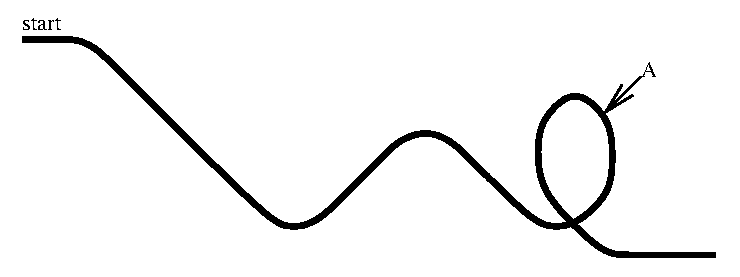
\includegraphics{../eps/roller_coaster.eps}

~ \vfill ~

\paragraph{Problem~\theproblem}\refstepcounter{problem}%
What formulae should go into cells E9 and F9 in this spreadsheet,
which is integrating a trajectory?\\
\resizebox{\textwidth}{!}{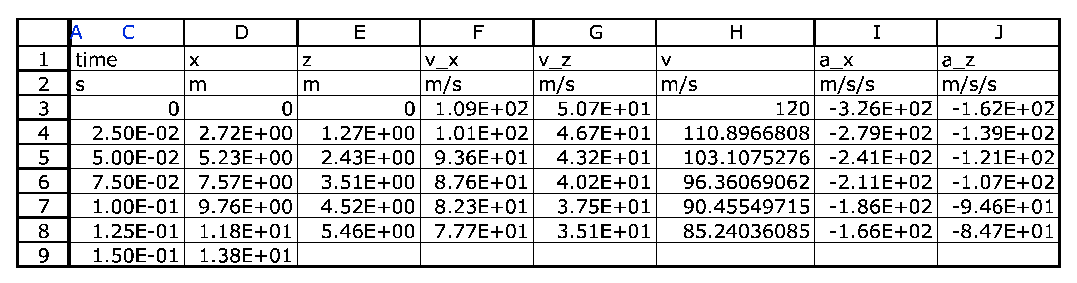
\includegraphics{../xls/exam.eps}}

~ \vfill ~

\clearpage

\paragraph{Problem~\theproblem}\refstepcounter{problem}%
How far does a typical American car have to drive before it has
``swept through'' a volume of air that has as much mass as the car
does?  If there are numbers of which you are uncertain, state your
assumptions.

~ \vfill ~

\paragraph{Problem~\theproblem}\refstepcounter{problem}%
A block of mass $m_2$ sits on top of a block of mass $m_1$.  The $m_1$
block is being pushed with a force $F$.  The ground is frictionless
but there is a coefficient of friction $\mu$ acting \emph{between} the
blocks.  For sufficiently large coefficient of friction, blocks $m_1$
and $m_2$ are stuck together.  In this limit, what is the magnitude of
the frictional force $F_\mathrm{f}$ between blocks $m_1$ and $m_2$?
To get full credit, \emph{make sure you draw free-body diagrams for
both blocks,} showing all forces acting (ignoring air resistance).
\marginpar{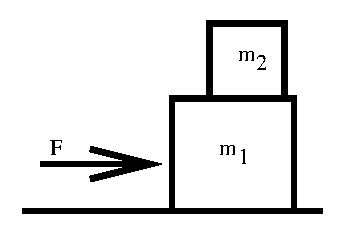
\includegraphics{../eps/stacked_blocks.eps}}%

~ \vfill ~

\clearpage

\paragraph{Problem~\theproblem}\refstepcounter{problem}%
A stone of mass $0.5\,\kg$ is thrown at a speed of $1\,\mps$ directly
downward.  How long does it take to travel downward $10\,\m$?  Ignore
air resistance.

~ \vfill ~

\paragraph{Problem~\theproblem}\refstepcounter{problem}%
In this block-and-pulley system, do you expect the $7\,\kg$ mass to
accelerate upwards, accelerate downwards, or not accelerate at all?
Consider the moment after it is released from rest.  Assume that the
masses of the ropes and pulleys are negligible, as is friction and air
resistance.  \emph{Hint:} Consider the case of just the $3\,\kg$ and
$4\,\kg$ blocks alone first.
\marginpar{\includegraphics{../eps/blocks_3_4_7.eps}}%

~ \vfill ~

\clearpage

\paragraph{Problem~\theproblem}\refstepcounter{problem}%
Pressure $P$ is a force per unit area, density $\rho$ is a mass per
volume, and local gravitational $g$ is an acceleration.  What
combination of these has units of length?  What might this length be?

~ \vfill ~

\paragraph{Problem~\theproblem}\refstepcounter{problem}%
A student of mass $80\,\kg$ stands at rest next to a block of ice of
mass $320\,\kg$, also at rest, on a frictionless frozen lake.  The
student pushes on the block until the block is moving away from the
student at $1\,\mps$ (that is, until
$\left|\vvice-\vvstudent\right|=1\,\mps$).  How much work did the
student do?  Give your answer in $\J$.  Don't forget to conserve
momentum!  \emph{Hint:} All that work went into kinetic energy.

~ \vfill ~

\clearpage

\paragraph{Problem~\theproblem}\refstepcounter{problem}%
The top graph shows the position $x(t)$ as a function of time for a
mass $m$ on a spring $k$, oscillating in the $x$ direction.  In the
next three graphs, plot the kinetic energy $K(t)$, the potential
energy $U(t)$, and the total mechanical energy $E=U+K$ for the mass as
a function of time.  \emph{Be sure to clearly label your graphs with the
minimum and maximum values the energies take on.}
\resizebox{\textwidth}{!}{\includegraphics{../pro/spring_energy.eps}}

\clearpage

\section*{Name:}

~ \vfill ~

This page intentionally left blank.

~ \vfill ~

\end{document}
